\documentclass{article}
\title{Obejektorientierte Datenbanken}
\author{Julius Dehner, Mohamad Aldirani}
\date{16.10.18}
\usepackage{graphicx}
\usepackage[utf8x]{inputenc}
\begin{document}
\maketitle



\section{Hintergrund}

Objektorientierte Datenbanken eignen sich gut für die Verwendung mit vielen Anwendungen.
\begin{itemize}
\item da sie auf Grund der ähnlichen Struktur mit Objektorientierten Programmiersprachen gut funktionieren
\item da sie multimediale Daten wie Bilder enthalten können
\end{itemize}
Dennoch werden häufig relationale Datenbanken eingesetzt, die anschließend in ein Objektorientiertes Modell übersetzt werden, da ODB häufig zu komplex sind.

\section{Definition}
In einer objektorientierten Datenbank werden Daten zusammen mit ihren zugehörigen Funktionen in einem Objekt gespeichert.

Ein Objekt modelliert normalerweise einen Gegenstand oder Begriff und enthält insbesondere dazugehörige Attribute; so gehört zum Beispiel die Farbe und das Gewicht eines Autos zu dem Objekt Auto. Attribute beschreiben ein Objekt näher. 

Essentiell ist hier, dass sich ein Objekt aus beliebigen anderen Datentypen zusammensetzt.

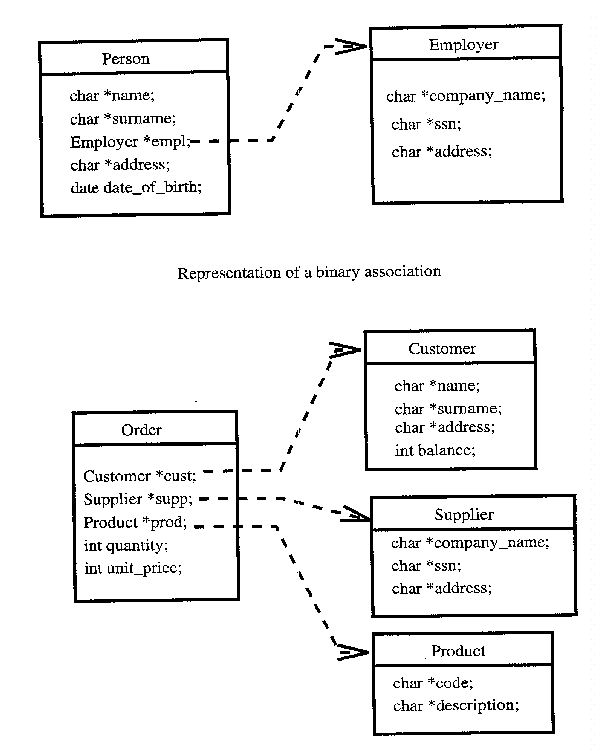
\includegraphics[scale=0.3]{Attributes.png}

Der Zugriff auf Daten funktioniert über das Parent-Child Modell, also kann beispielsweise durch Tür.Klinke.Farbe die Farbe einer Tür ausglesen werden.

Objektorientierte Datenbanken ähneln relationalen Datenbanken zunächst, doch durch die Inklusion von Methoden steigt die Komplexität der Datenbank stark an.

Diese Methoden haben verschiedenste Verwendungszwecke, wie umbenennen oder auch weitere Objekte zu erzeugen.


\section{Vor-/Nachteile}
\subsection{Vorteile}
\begin{itemize}
	\item Man kann beim Programmieren direkt mit Objekten arbeiten, statt Queries verwenden zu müssen
	\item Realtionen zwischen Daten werden durch objektorientierte Strukturierung klarer
	\item Eindeutige IDs werden automatisch für Objekte verteilt
\end{itemize}
\subsection{Nachteile}
\begin{itemize}
	\item Geringe Verbreitung
	\item Wenig Standartisierung
	\item Hohe Komplexität und eventuelle Performanceprobleme (auch durch mehrere mögliche Zugriffsarten auf Pfade)
\end{itemize}
\end{document}